% \chapter{Methoden und Praktiken}

\textit{In diesem Kapitel soll beschrieben werden, wie eine Nachvollziehbarkeit in Webapplikationen erreicht werden kann. Spezielle Methoden und Praktiken sollen vorgestellt und beleuchtet werden.}
% \textit{Hier könnte unter anderem \textbf{OpenTelemetry} betrachtet werden.}

\section{Methoden}

\subsection{Logging}

\textit{Folgende Fragen sollen zur Methode beantwortet werden}
\begin{enumerate}
	\item \textit{Gibt es Besonderheiten zu Logging in anderen Projekten (Backend vs. Frontend)?}
	\item \textit{Wie können Logs an einen auswertenden Stakeholder gelangen??}
	\item \textit{Welches Verhalten kann hiermit aufgedeckt/nachvollziehbar gemacht werden?}
\end{enumerate}

%\subsection{Monitoring}
%
%\textit{Folgende Fragen sollen zur Methode beantwortet werden}
%\begin{enumerate}
%	\item \textit{Welche Anwendungseigenschaften sind zu monitoren?}
%	\item \textit{Welches Verhalten kann hiermit aufgedeckt/nachvollziehbar gemacht werden?}
%\end{enumerate}

\subsection{Metriken}

\textit{Folgende Fragen sollen zur Methode beantwortet werden}
\begin{enumerate}
	\item \textit{Welche Metriken können definiert?}
	\item \textit{Wie können Metriken definiert werden?}
	\item \textit{Welches Verhalten kann hiermit aufgedeckt/nachvollziehbar gemacht werden?}
\end{enumerate}

\subsection{Tracing}

\textit{Folgende Fragen sollen zur Methode beantwortet werden}
\begin{enumerate}
	\item \textit{Welche Nutzerinteraktionen sind zu tracen?}
	\item \textit{Welches Verhalten kann hiermit aufgedeckt/nachvollziehbar gemacht werden?}
\end{enumerate}

\subsection{Fehlerberichte}

\textit{Folgende Fragen sollen zur Methode beantwortet werden}
\begin{enumerate}
	\item \textit{Was genau sind Fehlerberichte (=Bug-Reports) }
	\item \textit{Welches Verhalten kann hiermit aufgedeckt/nachvollziehbar gemacht werden?}
\end{enumerate}

\section{Werkzeuge und Technologien}

%\textit{Basierend auf dem Grundwissen über die Methoden und Praktiken, soll nun der Stand der Technik erörtert werden. Hierbei sollen Werkzeuge und Technologien und ihre Ansätze hervorgehoben werden und mit Hilfe welcher Methoden sie welches Ziel erreichen.}
%
%\textit{Wie in der Zielsetzung definiert sollen hier zwei bis drei Technologien näher vorgestellt werden.}
%
%\textit{Weiterhin könnte beleuchtet werden, wie ähnliche Herausforderungen bei anderen „Fat-Client“-Lösungen (also nicht SPAs) angegangen werden, und kann man hier vielleicht etwas lernen oder übertragen (und wenn nicht, warum nicht)?}

In der Fachpraxis haben sich einige Technologien über die Jahre entwickelt und etabliert, die eine verbesserte Nachvollziehbarkeit als Ziel haben. Es lassen sich zudem verschiedene Funktionskategorien festlegen, auf die sich die jeweiligen Technologien konzentrieren. Die einzelnen Technologien lassen sich jedoch nicht strikt kategorisieren und weisen unterschiedliche Funktionsumfänge für dieselben Kategorien auf. Deshalb werden die Kategorien folgend beschrieben, aber bei der Vorstellung der Technologien erfolgt keine Kategorisierung oder direkte Gegenüberstellung.

\subsection{Kategorien}

\subsubsection{System Monitoring}

System Monitoring beschäftigt sich mit der Überwachung der notwendigen Systeme und Dienste in Bezug auf Hardware- und Softwareressourcen. Es handelt sich hierbei um ein projektunabhängiges Monitoring, welches sicherstellen soll, dass die Infrastruktur funktionstüchtig bleibt.

\subsubsection{Log Management}

Log Management umfasst die Erfassung, Speicherung, Verarbeitung und Analyse von Logdaten von Anwendungen. Weiterhin bieten Werkzeuge hierbei oftmals Such- und Meldefunktionen.

\subsubsection{Application Performance Monitoring (APM)}

Beim Application Performance Monitoring werden Daten innerhalb von Applikationen gesammelt, die Rückschlüsse auf die Perfomanz von bspw. Transaktionen geben sollen \cite{StudyingTheEffectivenessOfAPMTools}. Mit diesen Daten können dann Regressionen der Performanz, in Aspekten wie Zeitaufwand oder Ressourcennutzung, festgestellt werden.

\subsubsection{Real User Monitoring (RUM)}

Real User Monitoring beschäftigt sich mit dem Mitschneiden von allen Nutzerinteraktionen mit bspw. einer Webapplikation. Hiermit lässt sich nachvollziehen, wie ein Nutzer die Anwendung verwednet. RUM kann dazu verwendet werden um Herauszufinden, wie ein Nutzer zu einem Zustand gelangt ist. Aber es können auch ineffiziente Klickpfade hierdurch festgestellt werden und darauf basierend UX Verbesserungen vorgenommen werden.

\subsubsection{Synthetic Monitoring}

Beim Synthetic Monitoring werden Endnutzerszenarien simuliert, um zu prüfen und sicherzustellen, dass diese Szenarien wie gewünscht ablaufen. Hierbei kann auf Aspekte wie Funktionalität, Verfügbarkeit und auch verstrichene Zeit kontrolliert werden.

\subsubsection{Tracing}

Tracing beschäftigt sich mit dem Aufzeichnen von Kommunikationsflüssen. Hierbei können einerseits die Kommunikationsflüsse innerhalb einer Applikation oder innerhalb eines Systems erfasst werden, aber auch andererseits die Kommunikationsflüsse bei verteilten Systemen erfasst werden, um diese meist komplexen Zusammenhänge zu veranschaulichen. Ein herstellerunabhängiger Standard, der sich aus diesem Gebiet entwickelt hat, ist OpenTracing \cite{OpenTracing}.

\subsubsection{Error/Crash Monitoring}

Das Error Monitoring konzentriert sich auf das Erfassen und Melden von Fehlern. Es werden oftmals neben dem eigentlichen Fehler auch Aspekte vom RUM und Logging gemeldet, um mehr Kontextinformationen zu liefern.

\subsubsection{Session Replay}

Session Replay bedeuted, dass eine Sitzung eines Nutzers nachgestellt wird, so als ob sie gerade passiert. Hierbei können einzelne Aspekte der Anwendung nachgestellt werden, bspw. der Kommunikationsablauf, bei dem die tatsächliche zeitliche Abfolge von Kommunikationen nachvollzogen werden können. Desto mehr Aspekte nachgestellt werden, desto realitätsnaher ist die Simulation und entsprechend hilfreich ist sie beim Nachvollziehen.

\subsection{Fachpraxis}

Bei der Recherche zu Werkzeugen und Technologien aus der Fachpraxis wurden eine Handvoll Produkte näher betrachtet. Folgend werden die Ergebnisse beschrieben, diese dienen aber nicht als Vergleich oder detaillierte Produktbeschreibung, eher wird ein grobes Verständnis der Fachpraxis gewonnen, um im Verlauf der Arbeit darauf zurückgreifen zu können. Bei dieser Recherche wurde immer wieder auf den Standard OpenTelemetry gestoßen, weshalb dieser zunächst kurz beschrieben wird.

\subsubsection{OpenTelemetry}

\begin{wrapfigure}[19]{r}{0.45\textwidth}
\centering
\vspace{-\baselineskip}
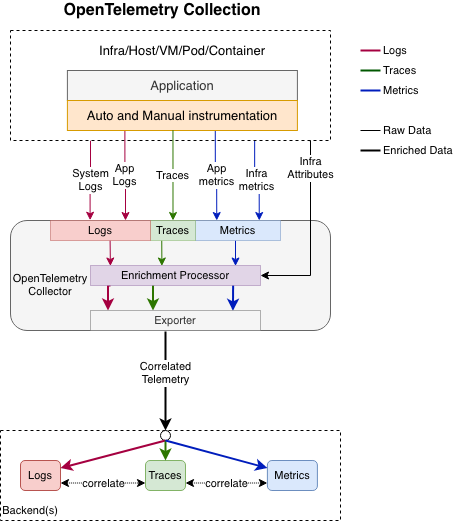
\includegraphics[width=\linewidth]{img/03_methoden/otel_unified-collection.png}
\caption{Schaubild einer Lösung auf Basis von OTel \cite{OpenTelemetryUnifiedCollection}}
\label{fig:otel-unified-collection}
\end{wrapfigure}

OpenTelemetry (OTel) \cite{OpenTelemetry} ist ein sich derzeit entwickelnder herstellerunabhängiger Standard, um Tracing-, Metrik- und Logdaten\footnotemark zu erfassen, verarbeiten, analysieren und zu visualisieren. Der Standard fasst die beiden Standards OpenTracing und OpenCensus \cite{OpenCensus} zusammen und hat sich als Ziel gesetzt diese zu erweitern. Hinter dem Standard stehen u. A. die Cloud Native Computing Foundation (CNCF), Google, Microsoft, und führende Hersteller in Tracing und Monitoring-Lösungen. Ein erster Release ist für Ende 2020/Anfang 2021 geplant. Ziel ist es, dass Entwickler Tools und Werkzeuge benutzen können, ohne jedesmal eine hochspezifische Anbindung schreiben und konfigurieren zu müssen. Stattdessen definiert der Standard Komponenten, die spezielle Aufgabengebiete haben und mit einer allgemeinen API angesprochen werden können. Die technische Infrastruktur einer auf OTel basierenden Lösung kann in \autoref{fig:otel-unified-collection} betrachtet werden. Im groben definiert OTel folgende Komponenten: API, SDK, Exporter, Collector und Backend (vgl. \autoref{fig:otel-components}).

\begin{figure}[H]
	\centering
	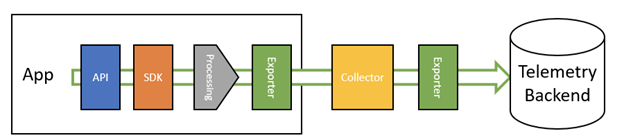
\includegraphics[width=0.75\linewidth]{img/03_methoden/dynatrace_otel-components.png}
	\caption{OTel Komponenten \cite{DynatraceOTelComponents}}
	\label{fig:otel-components}
\end{figure}

\nomenclature[Fachbegriff]{OTel}{OpenTelemetry}
\nomenclature[Fachbegriff]{CNCF}{Cloud Native Computing Foundation}
\footnotetext{Logging wird derzeit noch nicht unterstützt, es wird jedoch daran gearbeitet \cite{OpenTelemetryLoggingSpecification}}

\subsubsection{New Relic}

New Relic \cite{NewRelic} ist ein SaaS der gleichnamigen Firma, welcher Betreiber von Softwareprojekten dabei unterstützt das Verhalten ihrer Anwendungen zu überwachen. Der Dienst konzentriert sich auf System Monitoring, APM und RUM und erfasst die notwendigen Daten mit proprietären Lösungen. Neben den Kernfunktionalitäten unterstützt New Relic auch Log Management, Synthetic Monitoring, Tracing und Error Monitoring.

\nomenclature[Fachbegriff]{SaaS}{Software-as-a-Service}

Bei New Relic wurde die kostenlose Version aufgesetzt und evaluiert. Der New Relic Agent, welcher die Daten beim Client sammelt, wird über ein Skript eingebunden und sendet in regelmäßigen Abständen Daten an New Relic. Über die Oberfläche von New Relic können dann allgemeine Charakteristika der Clients betrachtet werden, wie Ladezeiten, Browserhersteller, Ajax-Antwortzeiten. Spezielle Eigenschaften eines einzelnen sind jedoch nicht möglich, wahrscheinlich u. A. aus Aspekten des Datenschutzes. Jedoch im Fehlerfall gibt es mehr Informationen, denn hier werden spezifische Daten (Stacktrace, genaue Browserversion, Uhrzeit, ...) zum Fehler sowie zum Client erhoben und in der Oberfläche dargestellt. Diese Informationen sind gut zum Nachvollziehen, dass ein Fehler aufgetreten ist und was die Rahmenbedingungen sind - jedoch sind die Informationen nicht ausreichend um ein klares Bild des Fehlers zu erhalten. Dies könnte mit dem Log-Management von New Relic komplementiert werden, jedoch wären diese selber erheben und an einen eigenen Server zu senden, um dann die Logs an New Relic weiterzuleiten. Des Weiteren wird der Agent standardmäßig von AdBlockern blockiert, sowie von der ``Enhanced Tracking Protection`` im Mozilla Firefox. Es ist nicht möglich New Relics Dienst selber zu hosten, es ist also eine sog. ``OnPremise``-Lösung nicht möglich, weiterhin wird auch eine Weiterleitung über einen eigens bereitgestellten Proxy nicht unterstützt.

New Relic gibt an, dass Daten nach dem OpenTelemetry Standard selber erfasst und an New Relic gesendet werden können, ohne eine proprietäre Software \cite{NewRelicAnnoundOTelBetaSupport}. Leider ist dieses Feature in der Testversion, die zum Evaluieren benutzt wurde, nicht enthalten und kann somit nicht bestätigt werden. Es sind jedoch offizielle und quelloffen veröffentlichte Exporter für New Relic verfügbar für .NET, Python und Java \cite{OpenTelemetryRegistry}.

\subsubsection{Dynatrace}

Dynatrace \cite{Dynatrace} ist ein SaaS des gleichnamigen Unternehmens, welcher Betreiber von Softwareprojekten dabei unterstützt das Verhalten ihrer Anwendungen zu überwachen. Der Dienst konzentriert sich auf System Monitoring, APM und RUM und erfasst die notwendigen Daten mit proprietären Lösungen, dem ``OneAgent``. Ganz ähnlich wie New Relic unterstützt Dynatrace neben den Kernfunktionalitäten auch Log Management, Synthetic Monitoring, Tracing und Error Monitoring.

Bei Dynatrace wurde die 14-tägige Testversion aufgesetzt und evaluiert. Wie zuvor genannt, erfolgt die Datenerhebung über den Dynatrace OneAgent, welcher genauso wie New Relics Agent kontinuierlich Daten sendet. Die Oberfläche von Dynatrace stellt auch ungefähr die selben Informationen dar wie New Relic, wobei Dynatrace das Ganze visuell ansprechender darstellt. Dynatrace bietet auch die Funktionalität vom Error Monitoring aber leidet unter demselben Problem wie New Relic: zu wenig Kontextinformationen.

Der Dynatrace OneAgent, wird standardmäßig von AdBlockern blockiert, aber nicht wie New Relic von der ``Enhanced Tracking Protection`` des Mozilla Firefox. Dynatrace kann zudem damit punkten, dass es als OnPremise-Lösung verfügbar ist, sodass Kunden genau bestimmen können, wo die Daten verarbeitet und gespeichert werden.

Dynatrace ist dem OpenTelemetry Team beigetreten und hat angegeben, an der Weiterentwicklung mitzuhelfen \cite{DynatraceJoinOTelProject}. Eine Integration des Dienstes Dynatrace ins Ökosystem von OTel gibt es jedoch noch nicht.

\subsubsection{Sentry}

Sentry \cite{Sentry} ist ein SaaS Produkt der Functional Software Inc, welches sich auf das Error Monitoring spezialisiert. Deshalb beschränken sich die Kernfunktionalitäten auf das Error Monitoring, auch wenn von anderen Gebieten einige Aspekte präsent sind, stellen diese keine eigens abgeschlossene Funktionalität dar.

Für Sentry wurde die kostenlose Version aufgesetzt und evaluiert. Sentry bietet bei NPM quelloffene Pakete an \cite{SentryJSGithub}, um Fehler zu erfassen und an Sentry zu melden. Es werden Pakete für folgende Frameworks bereitgestellt: JavaScript, Angular, AngularJS, Backbone, Ember, Gatsby, React und Vue. Das Aufsetzen stellt sich einfach dar und ermöglicht einige Konfigurations- und Verarbeitungsoptionen, bspw. können sensible Daten aus den Datenpaketen entfernt werden oder weitere Informationen gemeldet werden. Anders als bei den beiden vorherigen Tools wird zu Sentry nur kommuniziert, wenn ein Fehler auftritt. Hierbei werden dafür aber umso mehr Daten erhoben: Detaillierte Klickpfade des Nutzers, Logmeldungen der Browserkonsole sowie die Informationen, die auch die anderen Tools bereitstellen.

Gemeldete Fehler werden in ``Issues`` umgewandelt, welche einem Fehlerticket entsprechen und in der Oberfläche Funktionen zum Zuweisen und zum Nachhalten der Behebung bieten. Sentry versucht die eingetroffenen Fehler in bestehenden Issues zu gruppieren, sodass jeweils zusammengehörige Fehler auch zusammen behandelt werden. Bei Sentry fehlt die ganzheitliche Nachvollziehbarkeit, aber dafür sind die gesammelten Fehlerinformationen zahlreich und helfen beim Nachvollziehen.

Der Quellcode von Sentry wurde veröffentlicht und weiterhin wird bei Sentry auch eine OnPremise-Lösung, basierend auf Docker, angeboten \cite{SentrySelfHosted}.

\subsubsection{LogRocket}

LogRocket \cite{LogRocket} ist ein SaaS Produkt des gleichnamigen Unternehmens und konzentriert sich auf detailliertes Session-Replay von JavaScript-basierten Clientanwendungen, um Probleme zu identifizieren, zu nachvollziehen und lösen zu können. Session-Replay ist auch die einzig identifizierbare Kernfunktionalität, die LogRocket aufweist.

Für die Evaluierung wurde die kostenlose Testversion von LogRocket verwendet. Zur Datenerhebung wird das Paket \texttt{logrocket} von NPM hinzugezogen und nach der Initialisierung sammelt es eigenständig die notwendigen Daten. Mit Hilfe der gesammelten Daten wird die gesamte Sitzung des Nutzers nachgestellt, hierbei ist die Anwendung, den Nutzer und seine Aktionen, die Netzwerkaufrufe sowie das DOM zu sehen. Die Nachstellung wird video-ähnlich aufbereitet und erlaubt ein präzises Nachvollziehen der zeitlichen Reihenfolge und Bedeutung (vgl. \autoref{fig:logrocket-session-replay-example}).

Neben dem JavaScript SDK bietet LogRocket quelloffenene Plugins für folgende Bilbiotheken: Redux, React, MobX, Vuex, ngrx, React Native. LogRocket ist zudem als OnPremise-Lösung verfügbar. Zusätzlich bietet LogRocket auch einige Integrationen für andere Tools, wie z.B. Sentry. Die Integration mit Sentry wurde ebenso evaluiert, hierdurch wurde ermöglicht, dass von einem Sentry Issue direkt auf das Session-Replay des konkreten Fehlerfalls in LogRocket gesprungen werden konnte.

\begin{figure}[H]
	\centering
	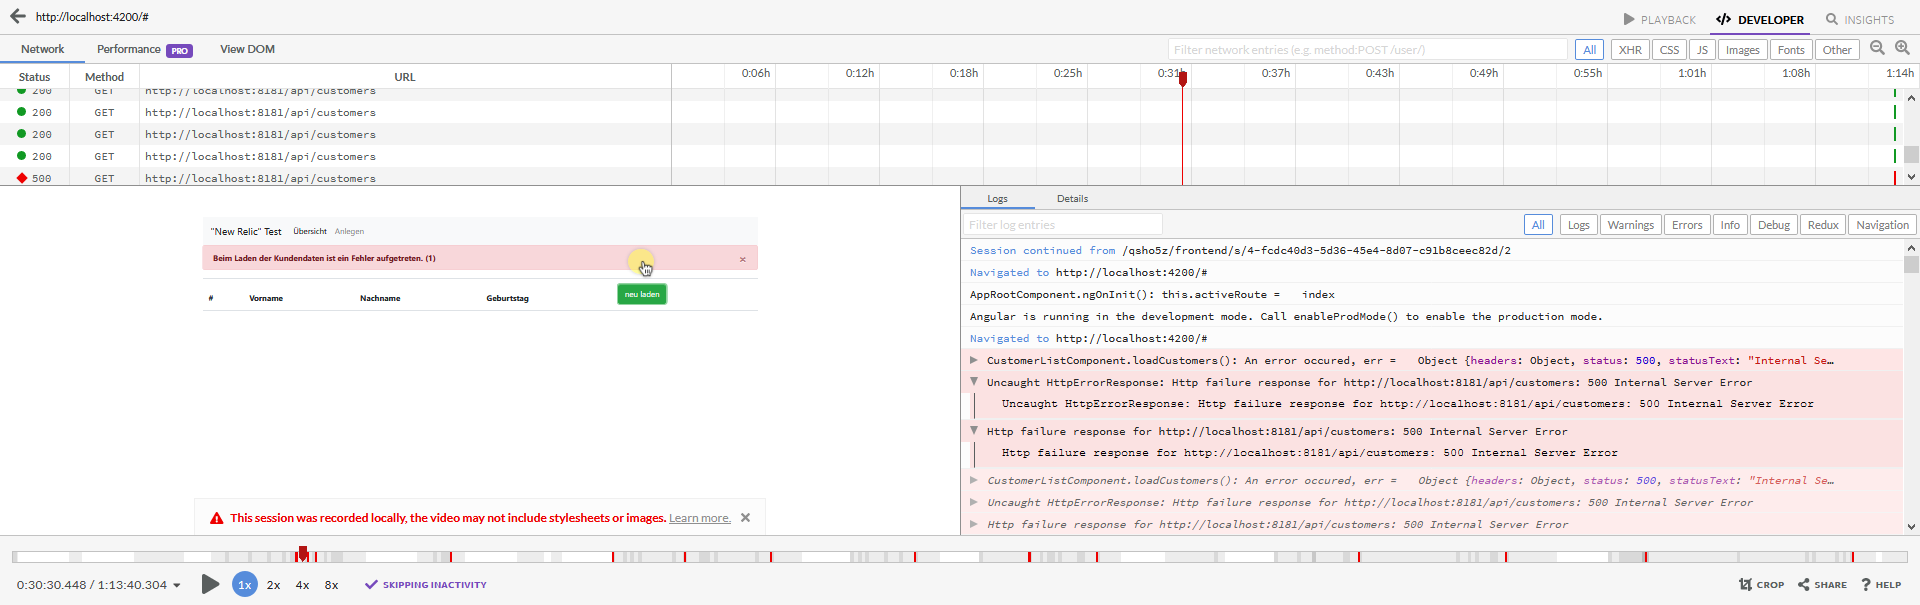
\includegraphics[width=\linewidth]{img/03_methoden/logrocket_session-replay-example.png}
	\caption{Beispiel eines Session-Replays bei LogRocket}
	\label{fig:logrocket-session-replay-example}
\end{figure}

\subsubsection{Splunk}

Splunk \cite{Splunk} ist ein Softwareprodukt und ein SaaS des gleichnamigen Unternehmens. Splunk fungiert als eine universelle Datensenke, sei es für Metriken, Logdaten o. Ä., und bietet Funktionen diese Daten zu durchsuchen, überwachen, analysieren und visualisieren. Splunk wird klassisch für Log Management eingesetzt, kann aber auch Aspekte von APM, RUM und Error Monitoring erfüllen.

Splunks kostenlose Version der SaaS wurde nur begrenzt evaluiert, denn schnell wurde festgestellt, dass das Daten senden vom Browserkontext zu Splunk nicht möglich ist, da Splunk mit ablehnenden CORS-Headern antwortet.

\subsubsection{Honeycomb}

Honeycomb \cite{Honeycomb} ist ein SaaS der Hound Technology Inc. und verspricht die Speicherung vieler (Tracing-)Daten und darauf basierend effiziente Abfragen zu ermöglichen. Es ist hauptsächlich als Tracingdienst anzusehen, womit jedoch auch Aspekte des APM, RUM und Error Monitoring mit abgebildet werden können.

Honeycomb wurde mit der kostenlosen Version evaluiert. Honeycomb bietet sog. ``Beelines`` an, welche Werkzeuge zur automatischen Datenerfassung sind. Diese Beelines sind aber nur für Node.js, Go, Python, Java, Ruby und Rails verfügbar, aber nicht JavaScript im Browser. Deshalb wurden zur Evaluierung Werkzeuge von OpenTelemetry hinzugezogen und zusätzlich musste nur noch ein Exporter für Honeycomb geschrieben werden. Honeycomb wirkt komplett anders als New Relic und Dynatrace, denn es ist nicht ausgefertigt mit konkreten Graphen und Darstellungen, sondern bietet eine Oberfläche mit dem man auf Basis der Daten selber Abfragen, Graphen und andere Darstellungen selber erstellen kann. Auch ist es nicht mit Jaeger, welches gleich näher betrachtet wird, vergleichbar, denn es bietet deutlich mehr Möglichkeiten als striktes Tracing.

\subsubsection{Jaeger}

Jaeger wurde 2017 als ein Projekt der CNCF gestartet \cite{Jaeger}. Es ist ein System für verteiltes Tracing von der Datensammlung bis hin zur Visualisierung, es unterstützt und implementiert den Standard OpenTracing.  Eine Unterstützung des OpenTelemetry Standards ist derzeit im Gange. Weiterhin kann Jaeger dazu benutzt werden, Metriken nach Prometheus \cite{Prometheus} zu exportieren, einem weiteren CNCF Projekt zur Speicherung und Visualisierung von Daten.

Jaeger wurde nicht aufgesetzt, sondern über Dokumentation und Kommunikation mit Kollegen der Open Knowledge evaluiert. Wie zuvor bei Honeycomb beschrieben, beschränkt sich Jaeger sehr auf Tracing, aber kann sich dafür auf dieses Gebiet spezialisieren und bietet eine gesamte Infrastruktur.

\subsubsection{Weiteres}

Bei meiner Recherche und Evaluierung wurden nicht alle auf dem Markt verfügbaren Werkzeuge und Technologien tiefergehend betrachtet. Deshalb werden weitere Funde, die nicht betrachtet wurden, hier kurz notiert:

\begin{itemize}
	\item APM \& RUM: AppDynamics, DataDog
	\item Error Monitoring: Airbrake, Instabug, Rollbar, Bugsnag, TrackJS
	\item Tracing: Google Cloud Trace, Zipkin
\end{itemize}

Auch diese Auflistung stellt nicht die komplette Bandbreite an Werkzeugen und Technologien dar und eine vorherige Betrachtung ist nicht als direkte Empfehlung zu verstehen.

\subsection{Literatur}